\chapter{Nghiên cứu tiền đề: Hệ thống GRACE}\label{chap:grace_baseline}

Chương này phân tích chi tiết hệ thống \textit{GRACE} (Graph-Reasoning Augmented Conversational Engine), nghiên cứu tiền đề của chính tác giả đã được công bố tại hội nghị quốc tế SOICT 2025 \cite{phan2025grace}. Thay vì chỉ tóm tắt lại nội dung bài báo, chương tập trung làm rõ từng thành phần kỹ thuật cụ thể và chỉ ra các giới hạn cấu trúc mà GRACE chưa giải quyết được, đây là cơ sở trực tiếp để đề xuất hệ thống ARGOS trong chương tiếp theo.

\section{Tổng quan kiến trúc GRACE}

GRACE được thiết kế theo mô hình hai giai đoạn công nghiệp tiêu chuẩn: Tạo ứng viên (Candidate Generation) và Xếp hạng lại (Re-ranking). Toàn bộ quy trình hoạt động theo cơ chế đường ống tĩnh (Static Pipeline) và không yêu cầu tinh chỉnh (fine-tune) trọng số của bất kỳ mô hình ngôn ngữ nào.

\begin{figure}[H]
    \centering
    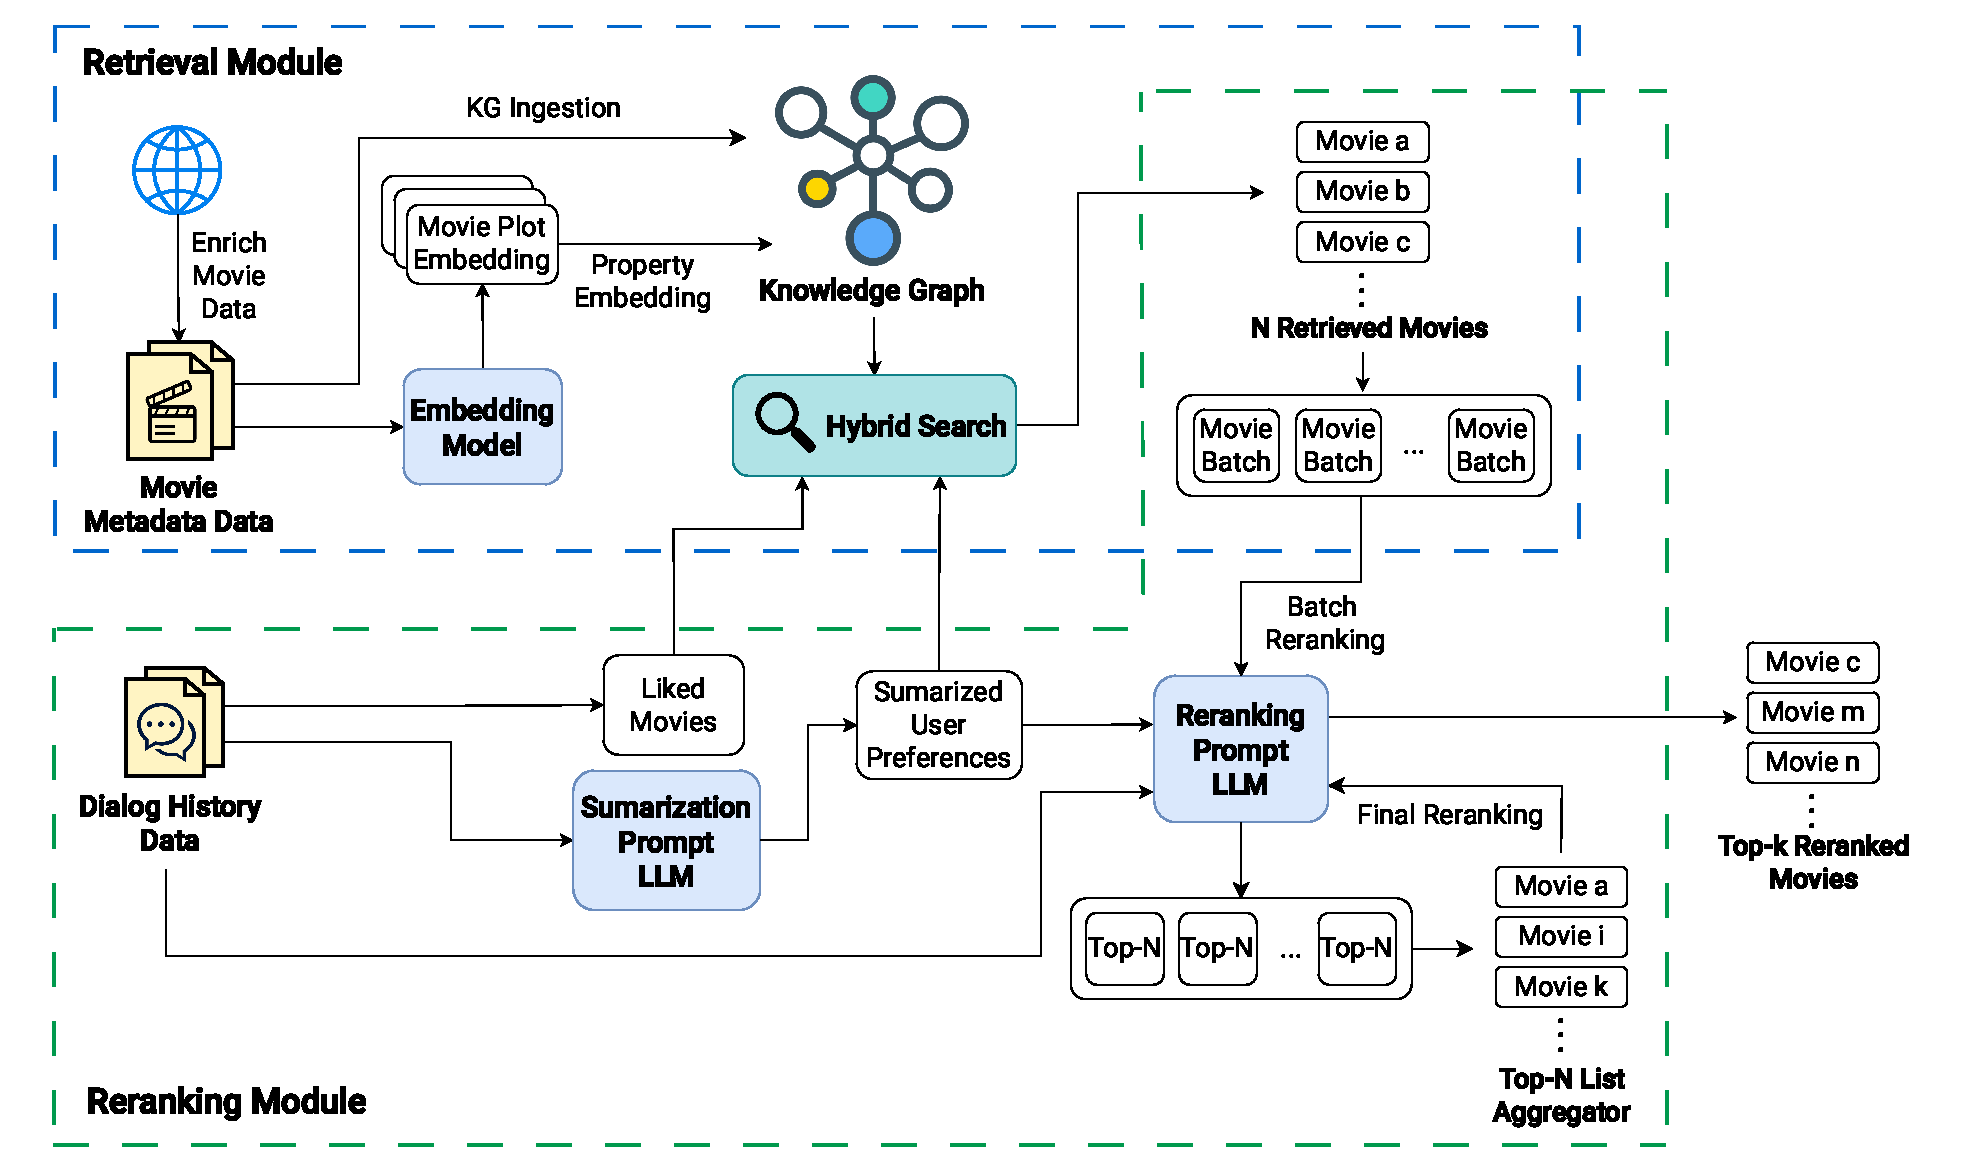
\includegraphics[width=\linewidth]{Chap3/images/grace.pdf}
    \caption{Tổng quan kiến trúc hệ thống tiền đề GRACE, bao gồm hai module chính: LLM Retriever và LLM Re-ranker.}
    \label{fig:grace_framework}
\end{figure}

Như minh họa trong Hình \ref{fig:grace_framework}, luồng hoạt động của GRACE gồm bốn bước tuần tự: (1) LLM tóm tắt lịch sử hội thoại thành một hồ sơ sở thích (Preference Profile); (2) ba chiến lược truy xuất song song (ngữ nghĩa, nội dung, đồ thị) tạo ra tập ứng viên; (3) các tập được hợp nhất và xếp hạng bằng Weighted Reciprocal Rank Fusion; (4) Generative LLM đánh giá lại và chọn ra kết quả cuối cùng. Kiến trúc này đảm bảo mọi thực thể trong tập ứng viên đều tồn tại trong KG vì chúng được truy xuất trực tiếp — loại trừ khả năng LLM tự bịa ra phim không tồn tại. Tuy nhiên, pipeline không kiểm tra liệu các ứng viên này có thỏa mãn toàn bộ ràng buộc cứng mà người dùng đặt ra trong hội thoại (danh sách loại trừ, ngưỡng điểm đánh giá) hay không — đây là khoảng trống mà Critic Agent trong ARGOS được thiết kế để lấp đầy.

\section{Xây dựng Đồ thị tri thức (Knowledge Graph Construction)}

Hiệu quả của GRACE phụ thuộc trực tiếp vào cấu trúc của Đồ thị tri thức (KG). Đồ thị này thống nhất siêu dữ liệu có cấu trúc và biểu diễn ngữ nghĩa cốt truyện vào cùng một không gian truy vấn.

\begin{figure}[H]
    \centering
    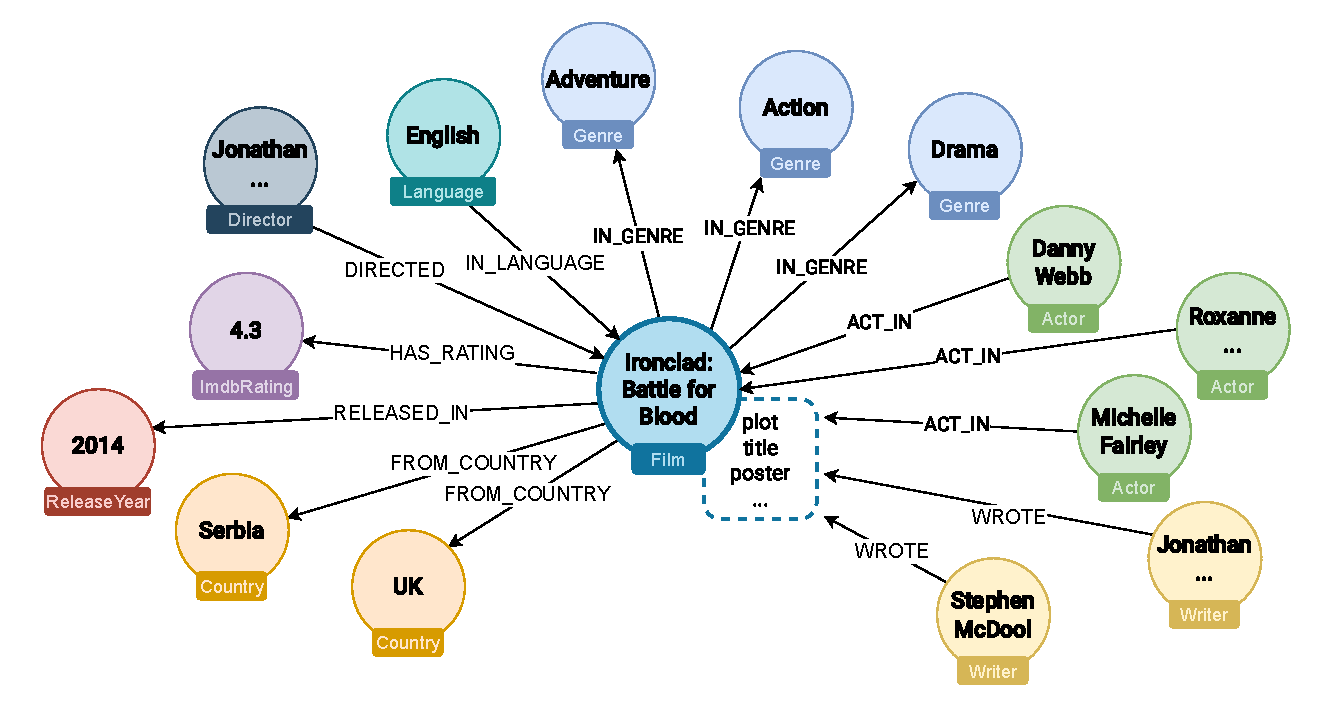
\includegraphics[width=0.85\linewidth]{Chap3/images/KG_node.pdf}
    \caption{Cấu trúc một node Phim (Film) trong Đồ thị tri thức. Node này liên kết trực tiếp với các thuộc tính (Năm, Điểm số, Thể loại) và các thực thể sáng tạo (Đạo diễn, Diễn viên).}
    \label{fig:kg_node}
\end{figure}

Quy trình xây dựng KG gồm ba bước:
\begin{itemize}
    \item \textbf{Tiền xử lý và Chuẩn hóa:} Chuyển đổi dữ liệu thô (năm phát hành, điểm số, thể loại, v.v.) sang định dạng sơ đồ thống nhất, xử lý các trường hợp nhập nhằng và trùng lặp thực thể.
    \item \textbf{Khởi tạo Đồ thị (Graph Construction):} Ánh xạ các thực thể phim và quan hệ vào cơ sở dữ liệu đồ thị Neo4j. Mỗi node Phim (\textit{Film}) được kết nối với các node phụ trợ như Thể loại (\textit{Genre}), Diễn viên (\textit{Actor}), Đạo diễn (\textit{Director}) (xem Hình \ref{fig:kg_node}).
    \item \textbf{Nhúng vector cốt truyện (Plot Embedding):} Gắn kèm vector nhúng dày đặc (dense embeddings) của đoạn tóm tắt cốt truyện trực tiếp vào node Phim tương ứng, cho phép truy vấn độ tương đồng cosine ngay bên trong đồ thị.
\end{itemize}

\section{Tóm tắt hội thoại và xây dựng Hồ sơ sở thích (Dialogue Summarization)}

Ký hiệu hội thoại đa lượt là $C = \{u_1, u_2, \dots, u_T\}$ với $u_t$ là phát ngôn thứ $t$. Mục tiêu của bước này là chưng cất $C$ thành một chuỗi văn bản tự nhiên duy nhất $\hat{P}$, gọi là Hồ sơ sở thích (Preference Profile), tóm tắt toàn bộ nhu cầu người tìm kiếm.

Thay vì dùng phương pháp điền khung (slot-filling) cứng nhắc với các trường có cấu trúc như \textit{likes, dislikes, constraints}, GRACE sử dụng một mẫu lời nhắc cố định \texttt{UserPreference} để buộc LLM sinh ra một đoạn văn xuôi mô tả duy nhất. Cách tiếp cận này tạo ra bản tóm tắt vừa đủ ngắn gọn, vừa dễ đọc, vừa thích hợp cho cả tìm kiếm từ khóa lẫn neo giữ vào KG, đồng thời giữ được tính chịu lỗi cao trước ngôn ngữ đời thường và hội thoại nhiễu.

\textit{Ví dụ từ tập dữ liệu ReDial:} cho đoạn hội thoại $C$ = [\textit{Respondent: "Hi, what kind of movies do you like?"}, \textit{Initiator: "I'm looking for a recommendation, I enjoyed A Nightmare on Elm Street (1984) when I was younger."}, \textit{Respondent: "Oh, you like scary movies?"}], LLM theo mẫu \texttt{UserPreference} sinh ra: $\hat{P}$ = \textit{"The seeker enjoys scary movies, particularly horror classics, and explicitly mentions A Nightmare on Elm Street (1984) as a movie they liked in the past. Their interest suggests a preference for suspenseful, frightening films, which can guide future recommendations."} Kết quả này cho thấy LLM không chỉ ghi nhận thực thể tường minh (tên phim) mà còn suy luận ra đặc trưng thể loại tiềm ẩn (genre affinity) từ ngữ cảnh.

Hồ sơ $\hat{P}$ sau đó được dùng làm đầu vào trực tiếp cho cả ba luồng truy xuất trong §\ref{sec:hybrid_retriever}.

\section{Module Truy xuất Lai (Hybrid Retriever)}\label{sec:hybrid_retriever}

Cơ chế truy xuất của GRACE kết hợp ba luồng độc lập để đảm bảo độ bao phủ (Recall) tối đa cho tập ứng viên, trong đó mỗi luồng bổ trợ cho nhau về loại thông tin khai thác được.

\subsection{Truy xuất ngữ nghĩa (Semantic Search)}
Hồ sơ sở thích được mã hóa thành vector truy vấn dày đặc $\mathbf{q}$, sau đó so sánh với vector cốt truyện $\mathbf{e}_f$ tại mỗi node phim trong KG qua độ tương đồng Cosine:
\begin{equation}
s_f = \cos(\mathbf{q}, \mathbf{e}_f) =
\frac{\mathbf{q} \cdot \mathbf{e}_f}{\lVert \mathbf{q}\rVert_2 \, \lVert \mathbf{e}_f\rVert_2}
\label{eq:similarity}
\end{equation}
trong đó $\lVert \mathbf{x} \rVert_2 = \sqrt{\sum_i x_i^2}$ là chuẩn Euclidean ($\ell_2$). Top-$m$ phim có $s_f$ cao nhất tạo thành tập kết quả $M_{\text{sem}}$. Luồng này đặc biệt hiệu quả khi nhu cầu người dùng mang tính chất thái, chủ đề hoặc cảm xúc khó biểu diễn bằng từ khóa cứng (Hình \ref{fig:semantic_retrieval}).

\begin{figure}[H]
    \centering
    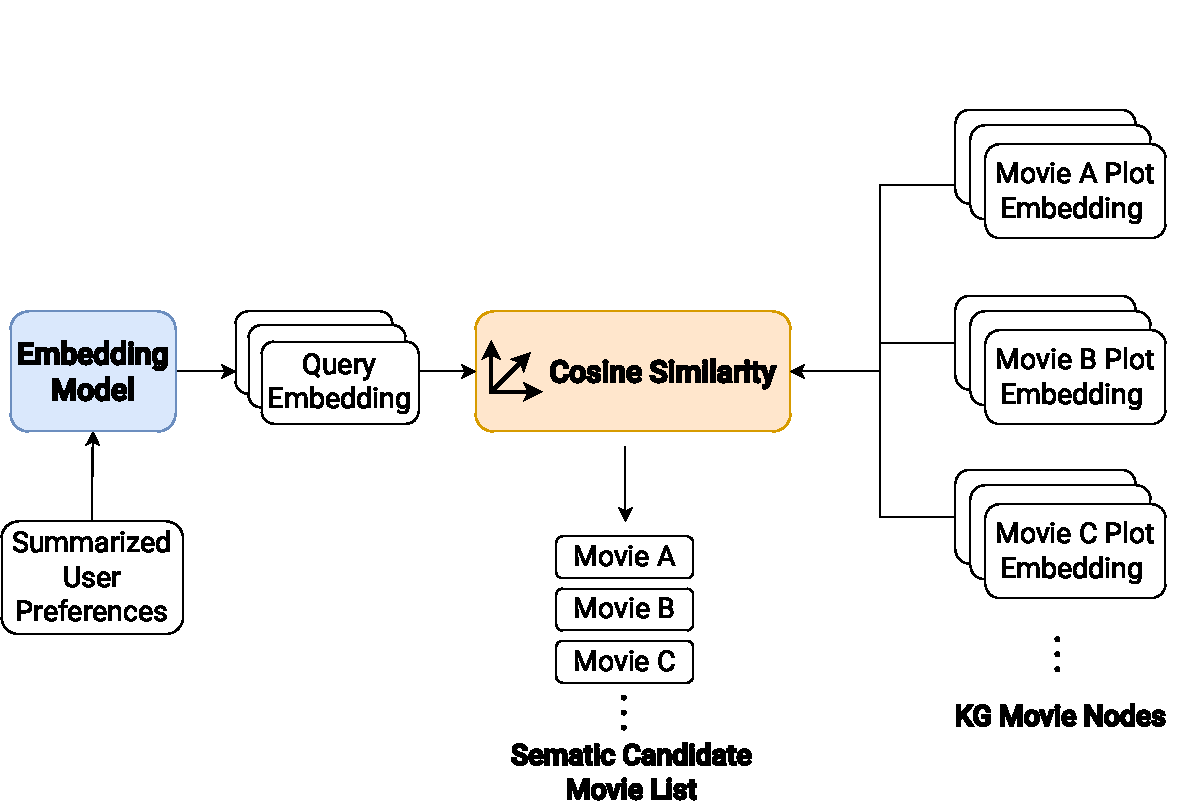
\includegraphics[width=0.85\linewidth]{Chap3/images/sem_retrieval.pdf}
    \caption{Quy trình truy xuất ngữ nghĩa dựa trên phép tính tương đồng Cosine giữa vector của câu truy vấn và vector cốt truyện phim.}
    \label{fig:semantic_retrieval}
\end{figure}

\subsection{Lọc theo nội dung (Content-based Filtering)}
Để thực thi các ràng buộc tường minh, ngữ cảnh hội thoại được chuyển đổi thành tập thể loại chuẩn hóa $G$ thông qua một bộ trích xuất LLM có ràng buộc (constrained LLM extractor), áp dụng ánh xạ từ đồng nghĩa (ví dụ: \textit{"science fiction"} $\mapsto$ \textit{"sci-fi"}), chuẩn hóa không phân biệt chữ hoa/thường, và chấp nhận nhãn ghép (compound labels). Khi $G$ không thể trích xuất đáng tin cậy, một bản đồ dự phòng keyword$\to$genre được dùng để đảm bảo độ phủ.

Mỗi phim $f$ với tập thể loại $\Gamma_f$ được đánh giá theo bộ giá trị xếp hạng từ điển (lexicographic tuple):
\begin{equation}
g_f = \big(|\Gamma_f \cap G|,\, r_f,\, y_f \big)\label{eq:enhanced_content_based}
\end{equation}
trong đó $|\Gamma_f \cap G|$ là số thể loại trùng khớp (ưu tiên tuyệt đối), $r_f$ là điểm IMDb, và $y_f$ là năm phát hành. Cách sắp xếp theo $y_f$ giảm dần mặc định ưu tiên phim mới hơn, một heuristic hợp lý trong phần lớn trường hợp nhưng có thể không phù hợp khi người dùng tìm phim cổ điển. Top-$m$ phim tạo thành tập $M_{\text{con}}$ (Hình \ref{fig:content_retrieval}).

\begin{figure}[H]
    \centering
    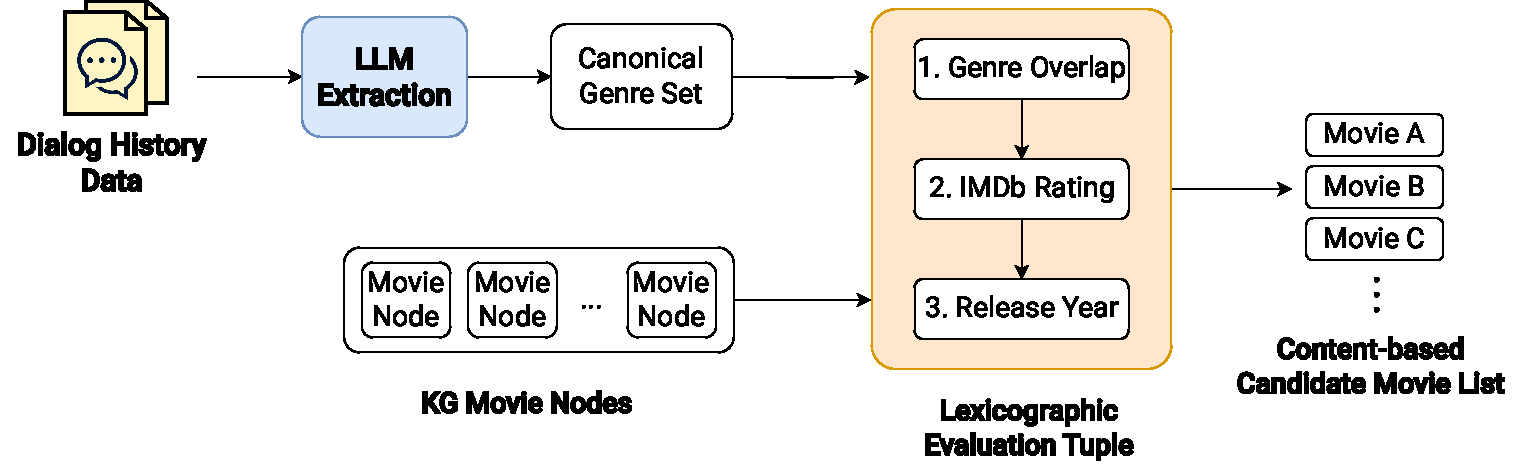
\includegraphics[width=0.85\linewidth]{Chap3/images/con_retrieval.pdf}
    \caption{Cơ chế lọc theo nội dung dựa trên các thuộc tính cứng (Thể loại, Năm sản xuất, Điểm số).}
    \label{fig:content_retrieval}
\end{figure}

\subsection{Mở rộng đồ thị (Graph Expansion - Collaborative)}
Xuất phát từ tập hạt giống (seed set) $L$ gồm các phim người dùng đã đề cập tích cực, thuật toán duyệt đồ thị dọc theo các cạnh liên kết với Diễn viên, Đạo diễn hoặc Biên kịch để tìm phim lân cận. Điểm số cộng tác cho phim ứng viên $f$ được tính:
\begin{equation}
S_{\text{col}}(f) = \sum_{s\in L} c(s,f) \label{eq:connection_count}
\end{equation}
trong đó $c(s,f)$ là số thực thể sáng tạo chia sẻ chung giữa phim hạt giống $s$ và phim ứng viên $f$. Các phim được sắp xếp theo tuple $\big(S_{\text{col}}(f), r_f\big)$ và top-$m$ tạo thành tập $M_{\text{col}}$ (Hình \ref{fig:collaborative_retrieval}).

\begin{figure}[H]
    \centering
    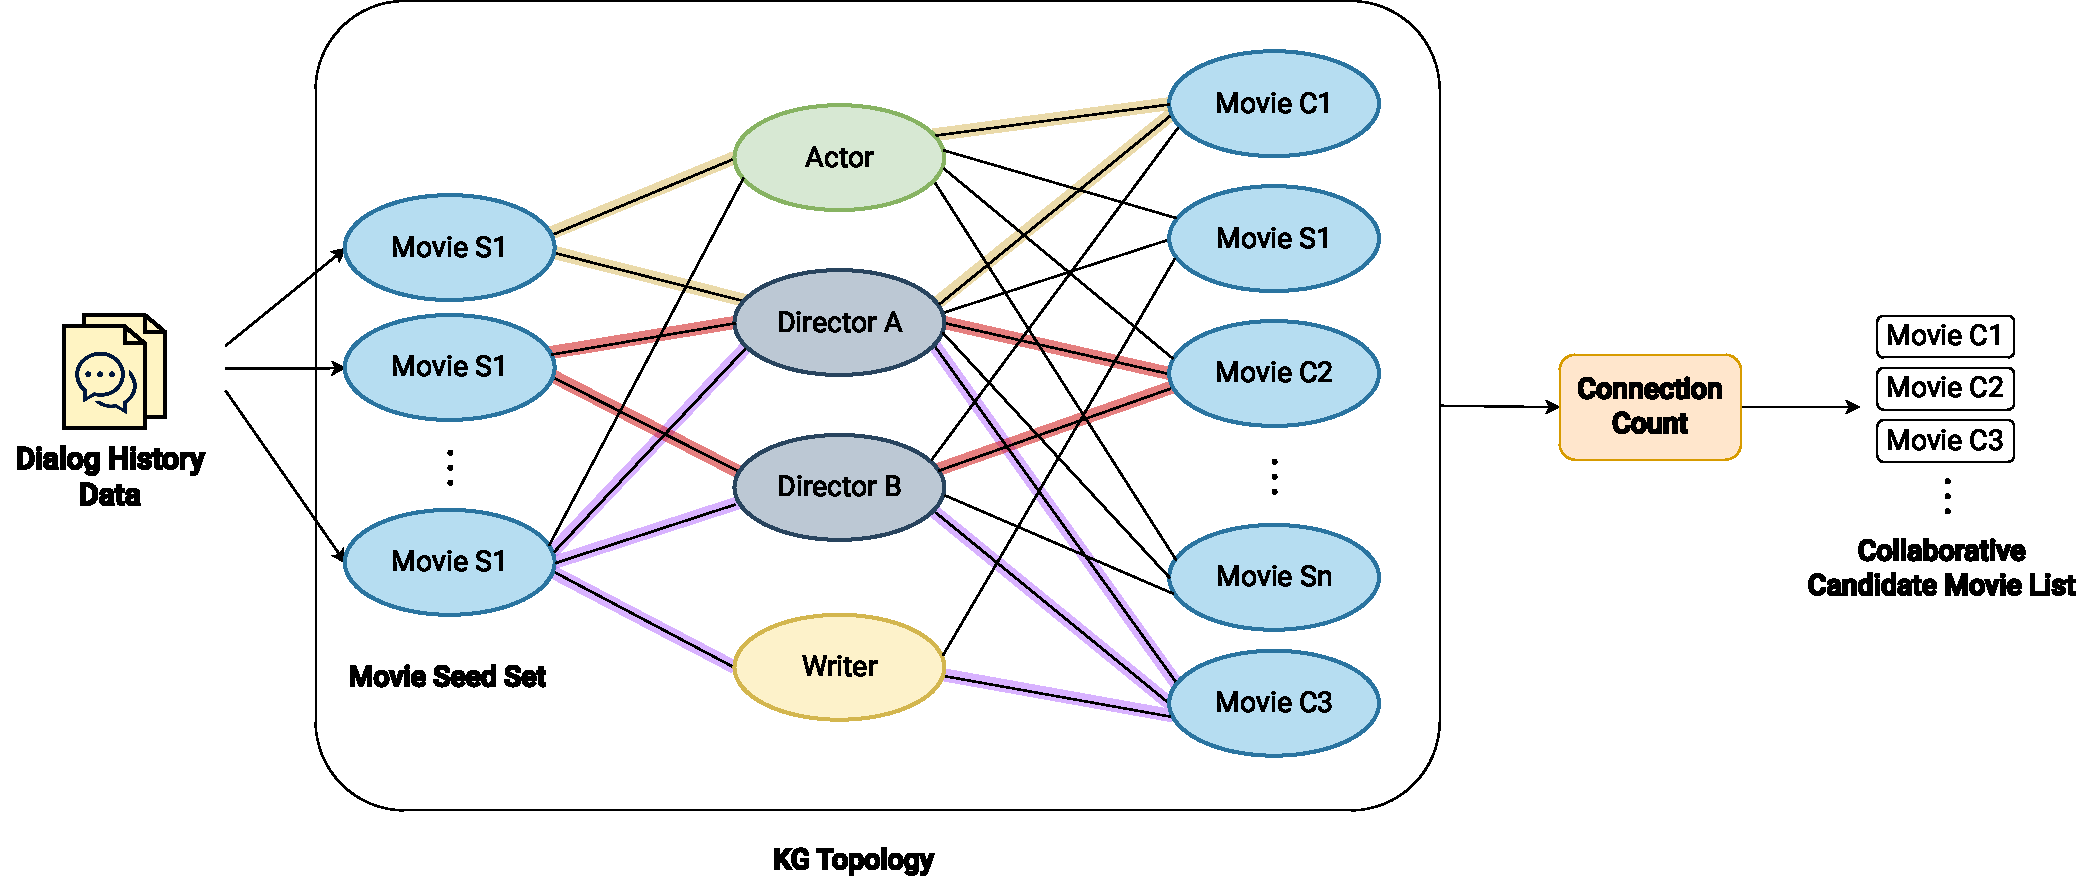
\includegraphics[width=0.85\linewidth]{Chap3/images/col_retrieval.pdf}
    \caption{Thuật toán mở rộng đồ thị dựa trên việc chia sẻ các node đội ngũ sáng tạo (Diễn viên, Đạo diễn).}
    \label{fig:collaborative_retrieval}
\end{figure}

\subsection{Cơ chế hợp nhất (Hybrid Integration)}
Đầu ra từ ba luồng trước tiên được gộp qua cơ chế loại bỏ trùng lặp ổn định (giữ nguyên thứ tự chèn):
\begin{equation}
M = \mathrm{StableDedup}(M_{\text{sem}} \cup M_{\text{con}} \cup M_{\text{col}})\label{eq:hybrid_integration}
\end{equation}
Tiếp theo, một bộ tiền xếp hạng tất định nhẹ (lightweight deterministic pre-ranker) theo thứ tự ưu tiên $(r_f, y_f)$ (điểm IMDb trước, năm phát hành sau) được áp dụng để lọc sơ bộ, loại bỏ ứng viên chất lượng thấp trước khi hợp nhất thứ hạng chính thức.

Các danh sách xếp hạng từ ba luồng sau đó được hợp nhất bằng thuật toán \textit{Weighted Reciprocal Rank Fusion} (WRRF) \cite{cormack2009reciprocal}:
\begin{equation}
\text{WRRF}(f) = \sum_{i \in \{\text{sem}, \text{con}, \text{col}\}} \frac{w_i}{k + \text{rank}_i(f)} \label{eq:wrrf}
\end{equation}
trong đó $w_i$ là trọng số của từng luồng (thực nghiệm: $w_{\text{sem}}=0.4$, $w_{\text{con}}=0.35$, $w_{\text{col}}=0.25$, được chọn để cân bằng giữa mức độ liên quan ngữ nghĩa, độ chính xác schema và đa dạng cộng tác), $\text{rank}_i(f)$ là thứ hạng của phim $f$ trong luồng $i$ (phim không có mặt được gán thứ hạng ảo lớn), và $k=60$ là hằng số làm mượt theo chuẩn RRF.

Đáng lưu ý, các trọng số $w_i$ được xác định thực nghiệm và \textit{cố định trong suốt quá trình vận hành}, bất kể hình thái ngôn ngữ của truy vấn. Đây là giới hạn thiết kế sẽ được phân tích tại §\ref{sec:grace_bottleneck}. Tập ứng viên cuối cùng $M_{\text{final}}$ được sắp xếp giảm dần theo điểm WRRF và chuyển giao cho module Re-ranker.

\section{Module Xếp hạng lại bằng Generative LLM}

Module Re-ranker (Hình \ref{fig:reranker}) nhận vào ba thành phần từ giai đoạn truy xuất: hồ sơ sở thích $\hat{P}$, tập ứng viên $M_{\text{final}}$, và siêu dữ liệu đã làm giàu (cốt truyện, thể loại, diễn viên, điểm số) của từng ứng viên. Cách tiếp cận này neo giữ quyết định của LLM vào thuộc tính thực chứng thay vì chỉ dựa vào ngữ cảnh hội thoại phẳng (flat dialogue context).

\begin{figure}[H]
    \centering
    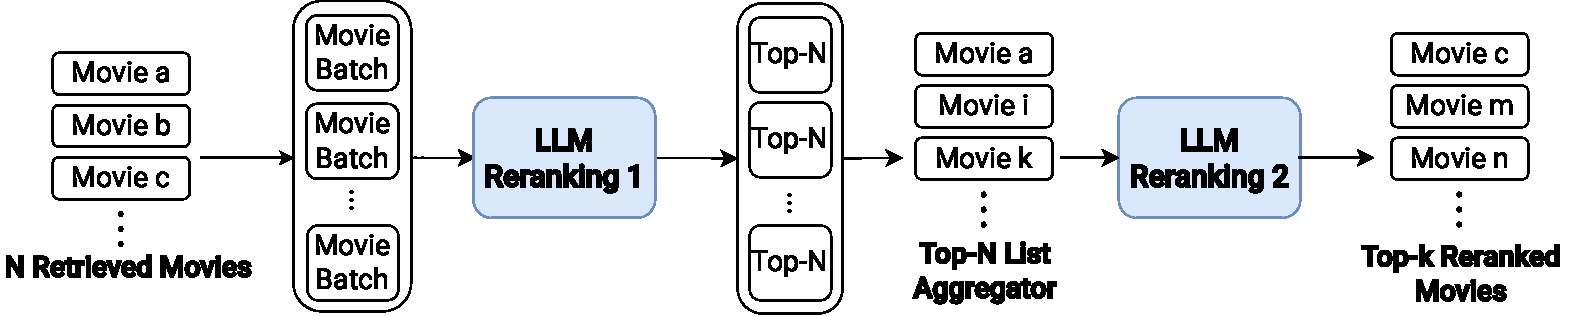
\includegraphics[width=0.85\linewidth]{Chap3/images/reranker.pdf}
    \caption{Kiến trúc Module Xếp hạng lại, sử dụng cơ chế batching để xử lý tập ứng viên lớn thông qua LLM.}
    \label{fig:reranker}
\end{figure}

Để xử lý giới hạn context window, GRACE giới thiệu kỹ thuật \textit{two-stage batching with shortlist fusion} kết hợp \textit{metadata augmentation}: (i) giai đoạn Batch Re-ranking chia $M_{\text{final}}$ thành các lô nhỏ, mỗi lô được LLM xếp hạng độc lập thành một shortlist; (ii) giai đoạn Final Re-ranking hợp nhất các shortlist và thực hiện một lượt đánh giá tổng hợp cuối để chọn ra top-K. Đây là kỹ thuật chưa được kết hợp đồng thời trong các hệ thống CRS trước đó như LLM-ReDial, UniCRS hay G-CRS.

Mô hình xuất ra một JSON object nghiêm ngặt chỉ chứa các phim từ tập ứng viên. Một validator độc lập kiểm tra tuân thủ schema, loại bỏ mục không hợp lệ, giải quyết trường hợp hòa (tie-breaking), và áp dụng cắt ngắn top-$k$ tất định. Cơ chế retry có giới hạn và sửa lỗi nhẹ đảm bảo hệ thống thoái hóa nhẹ nhàng (graceful degradation) thay vì thất bại hoàn toàn khi LLM trả về định dạng sai. Nhờ validator này, kết quả cuối cùng chỉ chứa các phim thuộc tập ứng viên đã được truy xuất từ KG — đảm bảo không có thực thể do LLM tự bịa ra. Giới hạn còn lại là validator chỉ kiểm tra tính hợp lệ schema của đầu ra, không đối chiếu ngược lại ràng buộc cứng của người dùng; điểm nghẽn này được giải quyết ở Chương 4.

\section{Phân tích điểm nghẽn mang tính cấu trúc}\label{sec:grace_bottleneck}

Mặc dù GRACE chứng minh được hiệu quả trong việc loại bỏ ảo giác và đạt kết quả cạnh tranh trên các bộ dữ liệu chuẩn (kết quả chi tiết tại Bảng \ref{tab:baseline_comparison}, Chương 5), kiến trúc Static Pipeline của nó bộc lộ ba điểm nghẽn có tính cấu trúc khi triển khai thực tế:

\begin{enumerate}
    \item \textbf{Tính phi linh hoạt của Pipeline (Pipeline Rigidity):} Luồng xử lý một chiều không có khả năng tự điều chỉnh khi một bước trung gian thất bại. Ví dụ điển hình: nếu LLM trong bước tóm tắt trích xuất nhầm thể loại từ hội thoại (diễn giải "phim căng thẳng" thành \textit{horror} thay vì \textit{thriller}), toàn bộ tập ứng viên từ luồng Content-based sẽ lệch hướng, nhưng pipeline không có cơ chế phát hiện và sửa lỗi này.

    \item \textbf{Thiếu điều phối trọng số động (Lack of Dynamic Weighting):} Trọng số WRRF cố định ($w_{\text{sem}}=0.4$, $w_{\text{con}}=0.35$, $w_{\text{col}}=0.25$) không phản ánh sự khác biệt về ngữ nghĩa giữa các loại truy vấn. Khi người dùng hỏi \textit{"phim gì có cùng diễn viên với Inception?"}, đây là truy vấn thuần đồ thị, do đó trọng số $w_{\text{col}}$ lẽ ra phải chiếm ưu thế tuyệt đối. Ngược lại, với yêu cầu \textit{"phim có không khí như Blade Runner"}, truy xuất ngữ nghĩa mới là kênh hữu ích. Pipeline tĩnh không phân biệt được hai tình huống này.

    \item \textbf{Chi phí và Độ trễ từ Generative LLM:} Việc dùng Generative LLM cho toàn bộ khâu re-ranking gây ra độ trễ đáng kể trong tương tác thời gian thực. Khi tập ứng viên lớn phải qua nhiều lô đánh giá, mỗi lô đều phát sinh một lần gọi API, tích lũy cả về chi phí lẫn latency, đặc biệt bất lợi khi cần phản hồi tức thì trong hội thoại.
\end{enumerate}

\section*{Kết luận chương}

Chương 3 đã phân tích chi tiết từng thành phần kỹ thuật của GRACE: từ cấu trúc KG, cơ chế tóm tắt hội thoại, ba luồng truy xuất lai, cho đến giai đoạn re-ranking bằng Generative LLM. Những thành tựu của GRACE trong việc loại bỏ ảo giác nhờ KG và cơ chế validator là cơ sở kỹ thuật quan trọng được ARGOS kế thừa. Tuy nhiên, ba điểm nghẽn được xác định (pipeline cứng nhắc, trọng số tĩnh và chi phí re-ranking) đặt ra yêu cầu rõ ràng cho kiến trúc kế tiếp: một hệ thống có khả năng tự điều chỉnh chiến lược và phản hồi nội bộ. Đây là nền tảng để Chương 4 trình bày kiến trúc đa tác tử \textbf{ARGOS}.
